% Charlotte Geiger - Manuel Lippert - Leonard Schatt
% Physikalisches Praktikum

% Teilauswertung X

\section{Umkehrdifferenzierer}
\subsection*{Vergleich der optimierten mit der nicht optimierten Schaltung}
Im folgenden wird diskutiert, inwiefern sich die Ausgangsspannung des Umkehrdifferenzierers ändert, wenn man die Grundschaltung aus Abbildung \ref{Differenzierschaltung} verwendet, 
oder wenn man Schaltung  verwendet.

\begin{center}
        \centering
        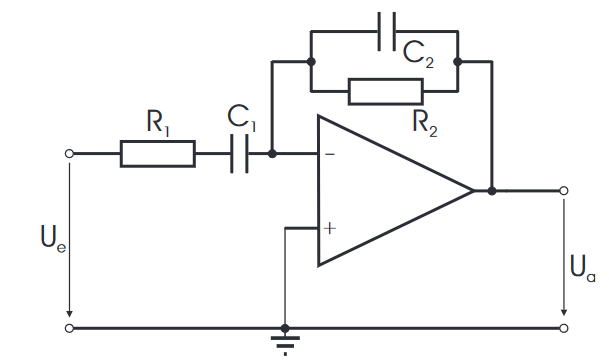
\includegraphics[width = 8cm]{diffOPV_verbessert.PNG}
        \captionof{figure}{Modifizierte Version eines Umkehrdifferenzierers}
        \label{modifiziertumkehrdiff}
\end{center} 
 
Wenn man das "differenzierte"  Bild der einfachen Schaltung \ref{Differenzierschaltung} betrachtet fällt einem sehr schnell auf, dass man einen Einschwingprozess wie in Grafik 
\ref{Einschwingprozess} beobachten kann. Dieser kommt daher, das die Schaltung nicht alles differenziert\footnotemark in dem Moment, in dem sich die Steigung sprunghaft ändert. 
Der Grund dafür ist, dass kein Wiederstand dem Kondensator $C_1$ vorgeschaltet ist. Bei hoher Frequenz ist der Widerstand des Kondensators sehr gering. Da der Innenwiderstand 
der Stromquelle nicht Null ist, fallen auch Teile der Spannung dort ab. 
\footnotetext{\url{file:///C:/Users/STUDIE~1/AppData/Local/Temp/Beschreibung%20Operationsverstarker.pdf}} 
Ein Teil des Signales wird undifferenziert durchgelassen. Dabei scheint dieser Prozess nicht bei allen Frequenzen im gleichen Maß abzulaufen. 
Man sieht, dass Eingangssignal von dem Funktionsgenerator erzeugt wird, eine komposition aus vielen Sinusspannungen zu sein scheint. Genauerer Informationen sollte man 
erhalten, wenn man das Ausgangssignal fouriertransformiert. 
Außerdem fällt auf, dass das Rauschen bei der Grundschaltung deutlich stärker ist, als bei der optimierten Schaltung.\\

\begin{figure}[h]
    \centering
    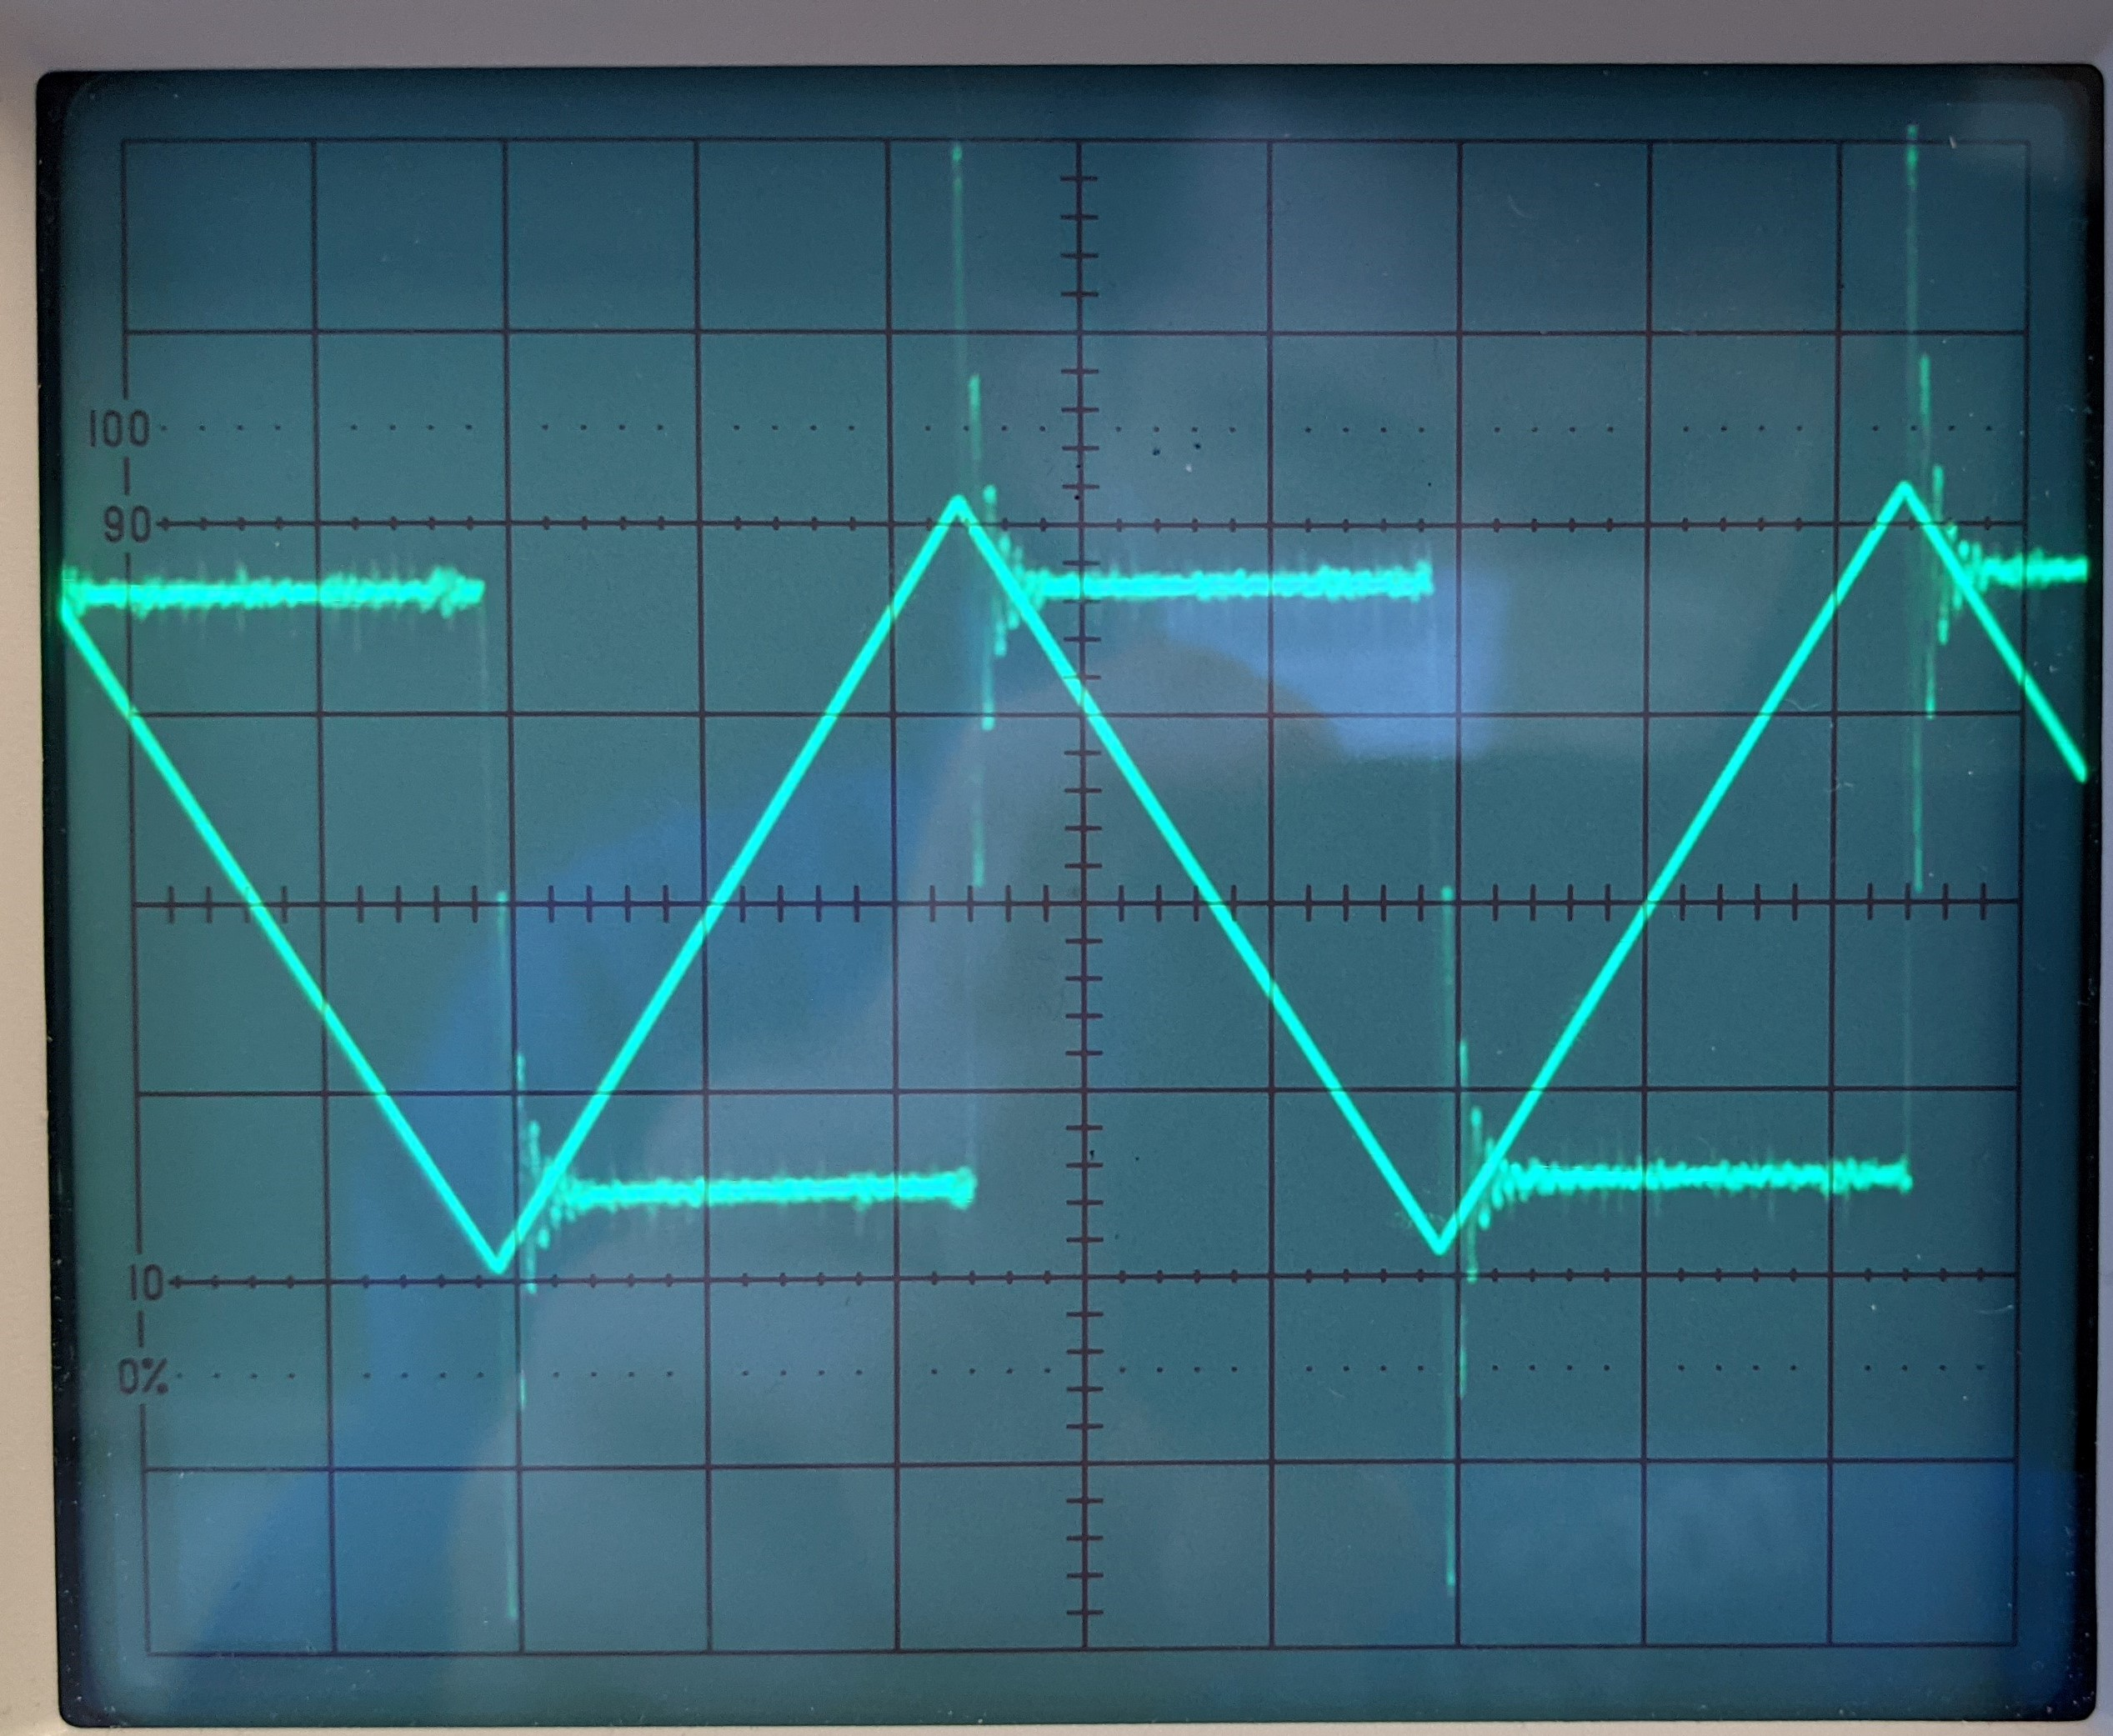
\includegraphics[width = 9cm]{Bilder/43-diffSchwingung.jpg}
    \caption{$U_a$ eines einfachen Umkehrdifferenzierers beim Anlegen einer Dreiecksspannung mit der Frequenz $f$ = 1kHz}
    \label{Einschwingprozess}
\end{figure}

Betrachten wir nun, dass die Ausgangssignal der modifizierten Schaltung aus Abbildung \ref{modifiziertumkehrdiff}. Dabei würden 
wir erwarten, dass das Rauschen stark vermindert wird, weil der Kondensator $C_2$ wie ein Teifpassfilter einfluss nimmt. Damit filtert er auch 
das Einschwingen sehr gut weg. Es bleibt der Gleichstromanteil in der Spannung.
\begin{figure}[h]
    \centering
    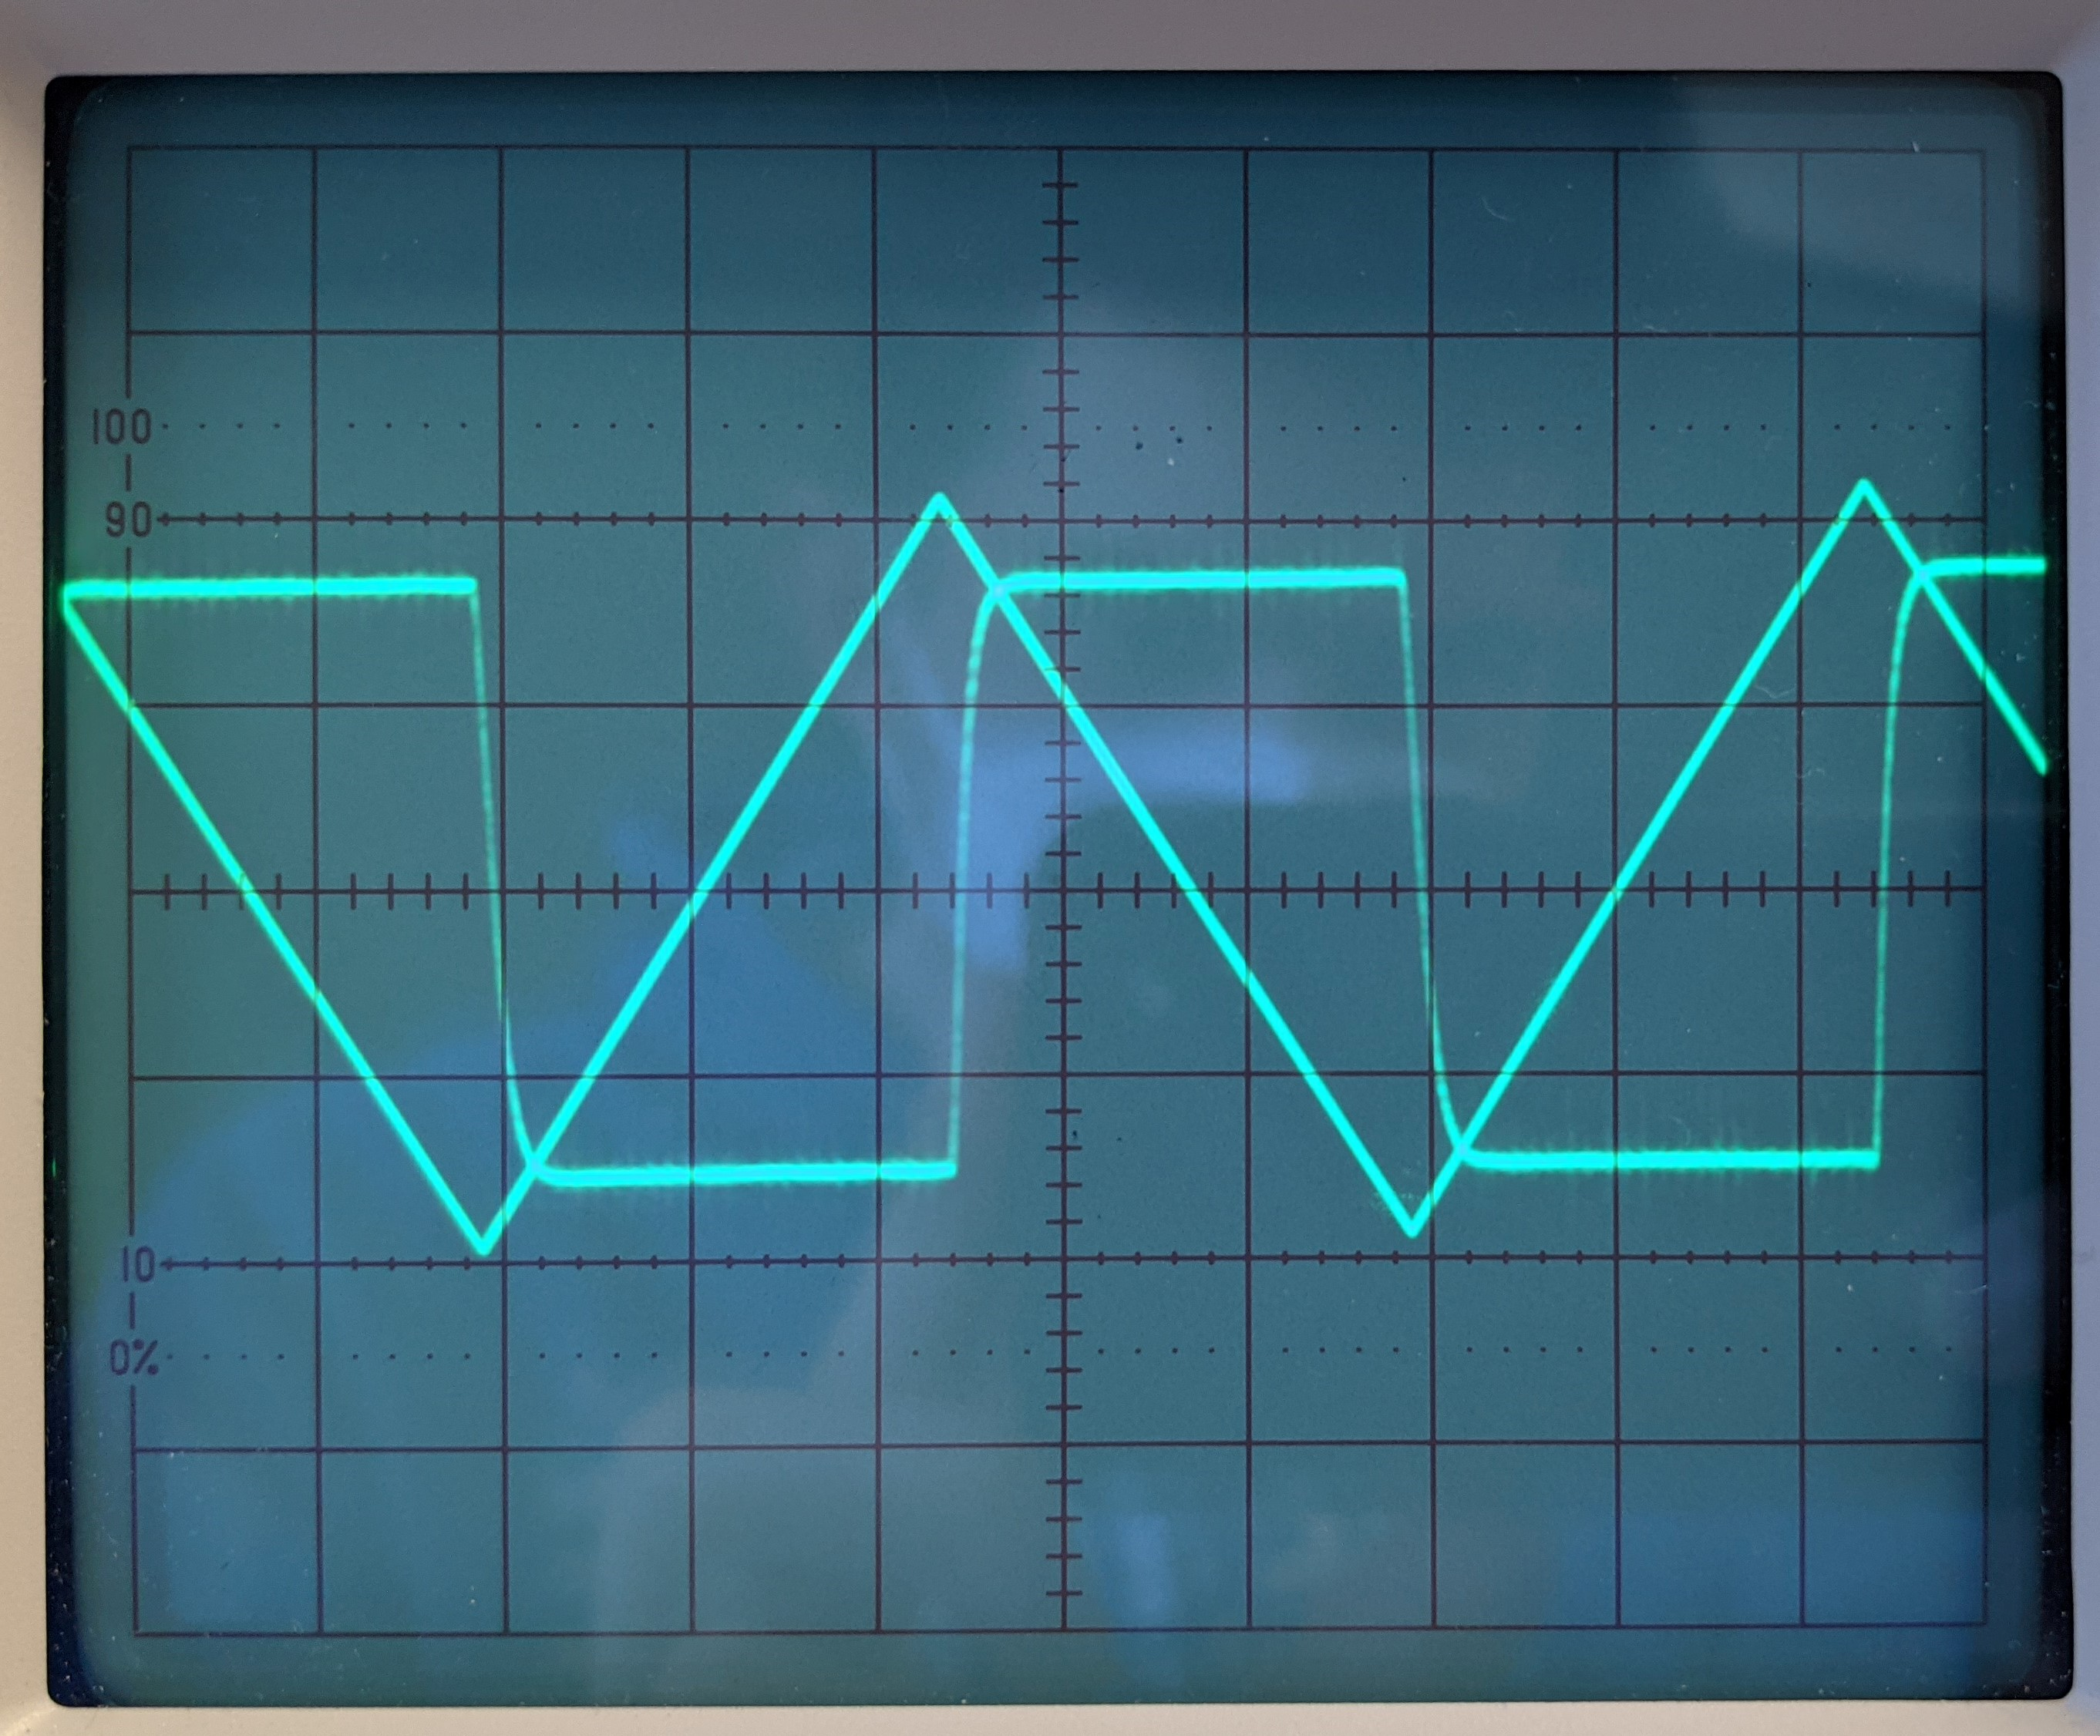
\includegraphics[width = 9cm]{Bilder/43-diffStabil.jpg}
    \caption{$U_a$ eines verbesserten Umkehrdifferenzierers beim Anlegen einer Dreiecksspannung mit der Frequenz $f$ = 1kHz}
    \label{Einschwingprozess}
\end{figure}
Das Differenzieren ist nicht perfekt, wegen der endlichen Flankenabfallzeit. Diese ist auf das Auf- und Entladen des Kondensators.

\section*{Zusammenhang zwischen dem Frequenzgang des Umkehrintegrators und dem des Umkehrdifferenzierers}
Im Folgenden werden die Verstärkung von Umkehrdifferenzierer und Umkehrintegrator in ein Diagramm aufgetragen. 
Diese schneiden sich bei $v = 1$.\\
Bevor wir den Frequenzwert $f$ jedoch betrachten, beschäftigen wir uns kurz mit der Theorie:\newline

\begin{gather*}
    v^{Integrator} = \frac{R_2}{R_1}\frac{1}{\sqrt{1+\omega ^2 R_{2}^2C_{2}^2}}\\
    f_{g}^{Integrator} = \frac{1}{2 \pi R_2 C_2}\\
    f_{T}^{Integrator} = konstant = f_{g}^{Integrator} \cdot v^{Integrator}(0) = \frac{1}{2\pi R_1 C_2 }\\
    s_{f_{T}^{Integrator}} = \sqrt{(\frac{s_{R_1}}{2 \pi R_{1}^2 C_2})^2+ (\frac{s_{C_2}}{2 \pi R_{1} C_{2}^2})^2}
\end{gather*}

Aus diesen Formeln mit den Bauteilen aus der vorherigen Aufgabe ergibt sich für unseren Aufbau hier:


\begin{center}
    \fbox{ $f_{T}^{Integrator} = (1,59 \pm 0,07) \mathrm{kHz}$}
\end{center}




Dieser Wert passt perfekt zu unserer Grafik (refer). %R
\newpage
\begin{figure}
    \centering
    %\includegraphics[width = \linewidth]{} #TODO #14 @ManeLippert
\end{figure}


Nun berechnen wir wie oben den selben Wert mit der Formel für den unmodifizierten Differenzierer aus den 
Fragen zur Vorbereitung.

\begin{gather}
    Abgelesen:\tab v  \overset{!}{=} 1\\
    v^{Differenzierer} = \frac{R_2}{R_1} \omega R_1 C_1\\
    \Rightarrow f_{T}^{Differenzierer} = \frac{1}{2 \pi R_2 C_1}\\
    s_{f_{T}^{Differenzierer}} = \sqrt{(\frac{s_{R_2}}{2 \pi R_{2}^2 C_1})^2+ (\frac{s_{C_1}}{2 \pi R_{2} C_{1}^2})^2}
\end{gather}

Setzen wir nun die von uns verbauten Teil ein, so folgt:

\begin{center}
    \fbox{ $f_{T}^{Differenzierer} = (1,59 \pm 0,07) \mathrm{kHz} = f_{T}^{Integrator}$}
\end{center}

An den Formeln sieht man sehr schön, dass sich der Schnittpunkt abhängig von der verbauten 
Bauteilen ändert.\\
Der Nachteil des Differenzierers ist, dass er für hohe Frequenzen instabil wird. Er differenziert nur 
wirklich gut im linearen niedrigfrequenten Bereich. Durch das vorschalten eines Widerstandes wird die Verstärkung begrenzt. 
Der zu $R_2$ parallelgeschaltete Widerstand bildet einen Hochpassfilter der Rauschen herausfiltern kann. 
Das führt dazu, dass die verbesserte Schaltung bei niedrigen Frequenzen wie ein Differentiator wirkt und bei hohen 
Frequenzen wie ein Verstärker mit ohmscher Rückkopplung.\footnotemark
\footnotetext{\url{https://www.electronics-tutorials.ws/de/operationsverstarker/differentiator-verstaerker.html}}
